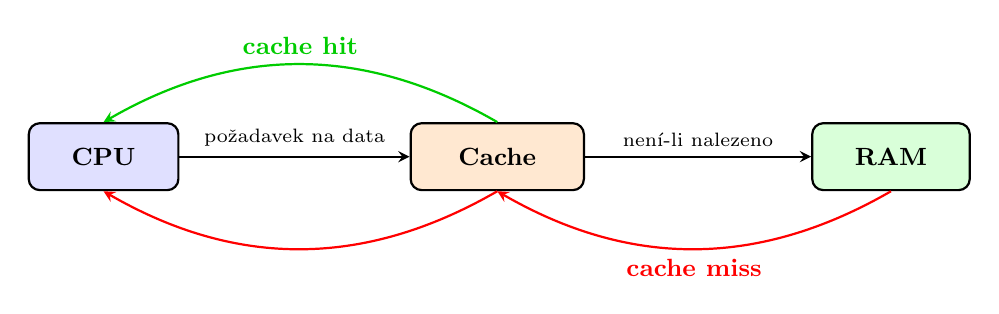
\begin{tikzpicture}[
    x=1cm, y=1cm,
    >=stealth,
    every node/.style={font=\small},
    mainbox/.style={
        draw,
        thick,
        rounded corners,
        align=center,
        minimum height=0.85cm
    },
    smallbox/.style={
        draw,
        thick,
        rounded corners,
        align=center,
        minimum height=0.65cm
    },
    arr/.style={->, thick}
]

    % Main path
    \node[
        mainbox,
        fill=blue!12,
        minimum width=1.9cm
    ] (cpu) at (-5.0,0.8) {\textbf{CPU}};

    \node[
        mainbox,
        fill=orange!18,
        minimum width=2.2cm
    ] (cache) at (0,0.8) {\textbf{Cache}};

    \node[
        mainbox,
        fill=green!15,
        minimum width=2.0cm
    ] (ram) at (5.0,0.8) {\textbf{RAM}};

    \draw[arr] (cpu.east) -- node[above, font=\scriptsize] {požadavek na data} (cache.west);
    \draw[arr] (cache.east) -- node[above, font=\scriptsize] {není-li nalezeno} (ram.west);

    \draw[arr,bend left=30,red] (ram.south) to node[midway,below] {\textbf{cache miss}} (cache.south);
    \draw[arr,bend left=30,red] (cache.south) to (cpu.south);

    \draw[arr,bend right=30,green!80!black] (cache.north) to node[midway,above] {\textbf{cache hit}} (cpu.north);

\end{tikzpicture}
